\documentclass{proc}

\usepackage{edbkps}
\usepackage{amsmath}
\usepackage{amssymb}
\usepackage{setspace}
\usepackage[utf8]{inputenc}
\usepackage{setspace}
\usepackage{subfig}
%%\usepackage[lined,boxed,commentsnumbered, linesnumbered]{algorithm2e}



\setcounter{secnumdepth}{2}
\setcounter{tocdepth}{0}
\let\footnote\savefootnote
\let\footnotetext\savefootnotetext
\let\footnoterule\savefootnoterule
\normallatexbib
\makeatletter
\renewcommand{\@ptsize}{0}
\makeatother

%%%%%
%% If you use a font encoding package, please enter it here, i.e.,
\usepackage{t1enc}


%%%%%
% Style for inserting .eps files and rotating illustrations or tables

% possible options for graphicx:
% [dvips], [xdvi], [dvipdf], [dvipsone], [dviwindo], [emtex], [dviwin],
% [pctexps],  [pctexwin],  [pctexhp],  [pctex32], [truetex], [tcidvi],
% [oztex], [textures]

\usepackage[dvips]{graphicx}
\usepackage[x11names, rgb]{xcolor}
\usepackage{tikz}
\usetikzlibrary{snakes,arrows,shapes}
\usepackage{amsmath}

%%%%%%%%%%%%%%%%%%%%%%%%%%%%%%%%%%%%%%%%%%%%%%%%%%%%%%%%%%%%%%%%%%%%%%%%%

\begin{document}


\articletitle[The Set Covering problem]
{Método do Volume Revisado para o problema Set Covering}

\author{João C. Abreu\altaffilmark{1}}

\altaffiltext{1}{Universidade Federal de Minas Gerais, DCC, \\
Avenida Antônio Carlos 6627, Belo Horizonte, Brazil,\\
\email{joao.junior@dcc.ufmg.br}}

\anxx{João C. Abreu Jr.,Universidade Federal de Minas Gerais\,
Avenida Antônio Carlos 6627\, Belo Horizonte\, Brasil\,
\emailfont{joao.junior@dcc.ufmg.br}}

\begin{abstract}
Esse relatório apresenta o algoritmo do volume revisado para o problema Set Covering.

\end{abstract}

\begin{keywords}
\inx{Set Covering}, \inx{Volume Revisado}
\end{keywords}

\doublespacing

\section{Introdução}
\label{sec:intro}

Dados $M=\{1,...,m\}$ e $N=\{1,...,n\}$ dois conjuntos. Seja $M_1$, $M_2$, ..., $M_n$ uma coleção de subconjuntos 
de $M$ com um custo $c_j$ associado a cada um desses subconjuntos. Uma cobertura de $M$ é um subconjunto 
$F \subset N$ tal que $\cup_{j \in F} M_j = M$. O problema que consiste em encontrar esse subconjunto $F \subset N$ de custo mínimo
é denominado o problema Set Covering($SCP$). Segundo Balas\cite{balas89} esse problema é $np$-$dificil$. \\
Para formular o $SCP$ como um problema
de otimização inteira, é introduzida uma matriz de incidência $A$ de tamanho $mxn$ para a coleção de subconjuntos 
$M_j, \forall j \in N$, com as entradas dadas por: \
\begin{align}
    & a_{ij} = \left \{\begin{array}{ll} 1; & \textrm{se } i \in M_j \textrm{,} \nonumber \\
    0; & \textrm{caso contrário} \nonumber
    \end{array}\right. \nonumber
\end{align}
A formulação para o $SCP$ proposta em \cite{Bertsimas05} é composta pela função objetivo \eqref{eq:objetivo1}
e pelas restrições \eqref{eq:ax1}-\eqref{eq:binarias}. Nessa formulação, a função objetivo \eqref{eq:objetivo1} minimiza o custo da cobertura procurada. 
Os valores constantes $c_j, \forall j \in N$ são os custos de cada subconjunto $M_j$. 
A variável de decisão $x_j$ é igual a $1$ quando $j \in F$ e $0$, caso contrário, onde $F \subset N$ é a cobertura procurada. \\
\begin{align}
    & \text{min } \sum_{j \in N} c_jx_j \label{eq:objetivo1} \\
    & \text{Sujeito à:} \nonumber \\
    & Ax \ge 1 \label{eq:ax1} \\ 
    & x \in \{0,1\}^n \label{eq:binarias}
\end{align}
O problema lagrangeano será composto pela associação dos multiplicadores as restrições em \eqref{eq:ax1} e ficará
como:
\begin{align}
    & \theta (\pi) = \text{min } \sum_{j \in N} c_jx_j + \pi(Ax -1) \label{eq:objetivo2} \\
    & \text{Sujeito à:} \nonumber \\
    & x \in \{0,1\}^n \label{eq:binarias1}
\end{align}

\section{Algoritmo}\label{sec:algoritmo} 
A figura \ref{AlgoritmoVolume} apresenta o algoritmo do volume revisado adaptado para o problema lagrangeano
$ \theta (\pi)$ retirado de \cite{Bahiense02}. 
\begin{figure}
\centering
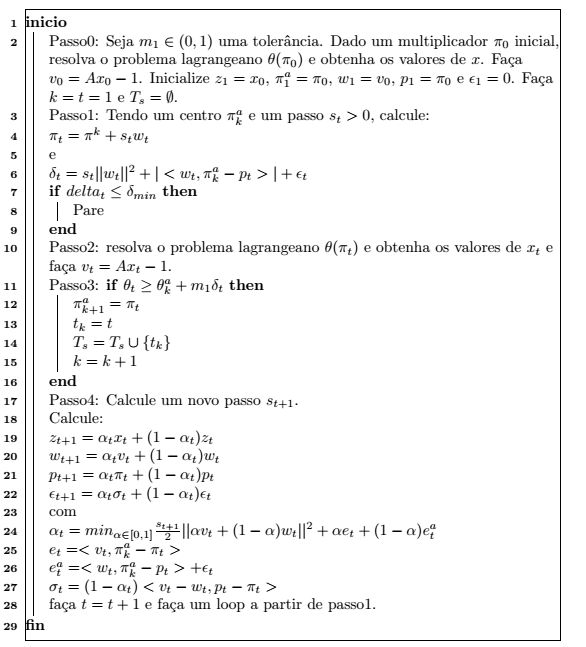
\includegraphics[width=4in]{AlgoritmoVolume.PNG}
\caption{Algoritmo do método do volume revisado para o problema lagrangeano $ \theta (\pi)$}
\label{AlgoritmoVolume}
\end{figure}

\section{Experimentos Computacionais}\label{sec:experimentos} 
Os experimentos computacionais foram executados em uma máquina Intel Dual-Core de 2.81 GHz de clock e
2GB de memória RAM, rodando o sistema operacional Linux. O modelo matemático composto pela função objetivo \eqref{eq:objetivo1} e
as restrições \eqref{eq:ax1}-\eqref{eq:binarias} foi implementado
no Ilog CPLEX 12.5.1 e o algoritmo da seção \ref{sec:algoritmo} foi implementado
em Python 2.7, sendo que o otimizador utilizado para resolver o problema lagrangeano $\theta (\pi)$ presente nesse algoritmo foi o Ilog CPLEX 12.5.1.
Foram utilizados quatro conjuntos de instâncias de testes nos experimentos computacionais e essas instâncias foram retiradas de \cite{Beasley90}.
Nessas instâncias de testes cada linha da matriz de incidência $A$ é coberta por pelo menos duas colunas e cada coluna cobre pelo menos uma linha. O
custo $c_j$ de cada coluna $j$ está entre $[1,100]$. A tabela \ref{table:instancias} resume esses conjuntos de instâncias. A coluna 1 dessa tabela 
representa o identificador do conjunto da instância de teste,
as colunas 2 e 3 mostram, respectivamente, o número $m$ de linhas e $n$ de colunas da matriz de incidência $A$. A coluna 4 representa
a densidade da matriz $A$ que é calculado pelo quantidade de 1's dessa matriz dividido pela quantidade total de elementos de $A$ que é igual a 
$mn$ e a coluna 5 mostra a quantidade de problemas em cada conjunto. Os dez problemas do conjunto 4 são nomeados como scp41-scp410, os cinco
problemas do conjunto 6 são nomeados como scp61-scp65, e os problemas do conjunto A e B são nomeados respectivamente como scpa1-scpa5
e scpb1-scpb5.

\begin{table}[htbp]
\begin{center}
  \begin{tabular}{|c|r|r|r|r|}
    \hline
      Conjunto & Linhas   & Colunas & Densidade   & Problemas\\ \hline
      4        & 200      & 1000    & 2           & 10 \\ \hline
      6        & 200      & 1000    & 5           & 5 \\ \hline
      A        & 300      & 3000    & 2           & 5 \\ \hline
      B        & 300      & 3000    & 5           & 5 \\ \hline
  \end{tabular}
\caption{Detalhes das instâncias de testes utilizadas}
\label{table:instancias}
\end{center}
\end{table}
No experimento desse trabalho foi comparado a performance do modelo matemático para o $SCP$ que será 
chamado aqui de $IP$, com o algoritmo proposto na seção \ref{sec:algoritmo}, que será chamado $VolumeRevisado$.
O modelo $IP$ foi executado através do CPLEX com todos os parâmetros default. O modelo presente no algoritmo $VolumeRevisado$
foi executado pelo CPLEX também com os valores default. O algoritmo $VolumeRevisado$ foi executado com os parâmetros 
$m_1 = 0.0001$, $\delta_{min} = 0.00001$, com um número máximo de iterações igual a 500000. O modelo $IP$ e o algoritmo $VolumeRevisado$ foram executados com um tempo de execução máximo de 7200 segundos. \\
A tabela \ref{table:resultados4e6} apresenta os resultados obtidos para o conjuntos de instância 4 e 6 e a tabela
\ref{table:resultadosaeb} apresenta os resultados para o conjuntos de instância A e B. Nessas tabelas a
coluna 1 mostra o nome da instância de teste, as colunas 2 e 3 são resultados referentes ao modelo $IP$ e as colunas
4,5 e 6 são resultados referentes ao algoritmo $VolumeRevisado$. A coluna 2 apresenta o custo da solução obtido pela
modelo $IP$ e a coluna 3 apresenta o tempo consumido para encontrar essa solução. A coluna 4 apresenta o custo da solução 
obtido pelo algoritmo $VolumeRevisado$, a coluna 5 traz o número de iterações do algoritmo
e a coluna 6 mostra o tempo consumido pelo algoritmo $VolumeRevisado$.\\
Para todas as instâncias do conjunto 4 e 6 o CPLEX conseguiu encontrar soluções ótimas em um tempo muito pequeno, conforme
pode ser observado pelas colunas 2 e 3 da tabela \ref{table:resultados4e6}. Para as instâncias scp41, scp46 e scp410 o algoritmo
$VolumeRevisado$ parou com uma solução de custo muito próxima da solução do modelo matemático, conforme
pode ser observado na coluna 4, linhas 1,6 e 10 da tabela \ref{table:resultados4e6}.

\begin{table}[htbp]
\begin{center}
  \begin{tabular}{|c|r|r|r|r|r|}
    \hline
      Instância & \multicolumn{2}{|c|}{$IP$} & \multicolumn{3}{|c|}{$VolumeRevisado$}\\
                & Custo Solução    & Tempo(s)  & Custo Solução   & \#Iterações & Tempo(s)      \\ \hline
      scp41     & 429              & 0.84      & 428.21          & 38       & 7.84       \\ \hline
      scp42     & 512              & 0.85      & 492.33          & 35436    & 7200.00       \\ \hline
      scp43     & 516              & 0.86      & 479.98          & 34061    & 7200.00       \\ \hline
      scp44     & 494              & 0.86      & 480.21          & 34520    & 7200.00     \\ \hline
      scp45     & 512              & 0.85      & 499.30          & 35192    & 7200.00       \\ \hline
      scp46     & 560              & 0.89      & 559.10          & 41       & 8.24    \\ \hline
      scp47     & 430              & 0.83      & 295.89          & 34368    & 7200.00       \\ \hline
      scp48     & 492              & 0.97      & 467.75          & 34983    & 7200.00    \\ \hline
      scp49     & 641              & 0.90      & 443.61          & 34813    & 7200.00    \\ \hline
      scp410    & 514              & 0.90      & 513.06          & 31       & 6.31    \\ \hline
      scp61     & 138              & 1.23      & 105.98          & 34797    & 7200.00    \\ \hline
      scp62     & 146              & 2.06      & 76.75           & 35879    & 7200.00    \\ \hline
      scp63     & 145              & 1.26      & 83.10           & 35389    & 7200.00    \\ \hline
      scp64     & 131              & 0.96      & 127.38          & 35493    & 7200.00    \\ \hline
      scp65     & 161              & 1.94      & 118.19          & 35540    & 7200.00    \\ \hline
  \end{tabular}
\caption{Comparação entre os custos da solução e tempos obtidos entre o modelo $IP$ e o algoritmo $VolumeRevisado$ para as instâncias do conjunto 4 e 6.}
\label{table:resultados4e6}
\end{center}
\end{table}

Para todas as instâncias do conjunto A e B o CPLEX conseguiu encontrar soluções ótimas em um tempo pequeno, conforme
pode ser observado pelas colunas 2 e 3 da tabela \ref{table:resultadosaeb}. Para essas instâncias o algoritmo {$VolumeRevisado$}
não conseguiu encontrar a solução ótima ou próxima da ótima para nenhuma delas, conforme pode ser observado pela coluna 4 da 
tabela \ref{table:resultadosaeb}.
\begin{table}[htbp]
\begin{center}
  \begin{tabular}{|c|r|r|r|r|r|}
    \hline
      Instância & \multicolumn{2}{|c|}{$IP$} & \multicolumn{3}{|c|}{$VolumeRevisado$}\\
                & Custo Solução    & Tempo(s)  & Custo Solução   & \#Iterações & Tempo(s)      \\ \hline
      scpa1     & 253              & 9.95      & 153.88          & 9859     & 7200.00  \\ \hline
      scpa2     & 252              & 9.87      & 209.80          & 10010    & 7200.00  \\ \hline
      scpa3     & 232              & 9.48      & 208.89          & 9804     & 7200.00 \\ \hline
      scpa4     & 234              & 8.76      & 207.49          & 10025    & 7200.00  \\ \hline
      scpa5     & 236              & 8.64      & 186.64          & 10006    & 7200.00 \\ \hline
      scpb1     & 69               & 10.08     & 55.89           & 10078    & 7200.00  \\ \hline
      scpb2     & 76               & 10.87     & 45.80           & 9867     & 7200.00  \\ \hline
      scpb3     & 80               & 9.67      & 55.92           & 9820     & 7200.00  \\ \hline
      scpb4     & 79               & 11.52     & 66.59           & 10024    & 7200.00  \\ \hline
      scpb5     & 72               & 9.86      & 53.16           & 10012    & 7200.00  \\ \hline
  \end{tabular}
\caption{Comparação entre os custos da solução e tempos obtidos entre o modelo $IP$ e o algoritmo $VolumeRevisado$ para as instâncias do conjunto A e B.}
\label{table:resultadosaeb}
\end{center}
\end{table}













Todo código fonte produzido por esse trabalho pode ser obtido no endereço eletrônico: $https://github.com/joaojunior/volume\_revisado2scp$

\bibliographystyle{plain}
%chapbblname{tp}  % The name of the .bbl file, what is normally the name of your .tex file.
\bibliography{tp} %\chapbibliography{gow}

\end{document}





% LocalWords:  comeca ij kj ji lll hardcoded eq ranqueamento recuperável RRSP
% LocalWords:  Recuperável Rent Minmax Regret Single Pair MSP SPP Cplex
